\chapter{Трансформерные модели}
\label{chap:transformers}

\begin{supportbox}{Об этой главе}
Свёрточные модели являются сильными базовыми моделями, особенно для изображений и последовательностей, где преобладают локальные отношения, но они ограничены в обработке очень длинных последовательностей или нелокальных зависимостей между элементами последовательности. В этой главе мы представляем другой класс моделей, называемых трансформерами, которые предназначены для преодоления таких проблем.
\end{supportbox}

\section{Длинные свёртки и нелокальные модели}

После ключевых разработок в период 2012-2016 годов, обсуждавшихся в предыдущей главе, следующий важный прорыв в проектировании дифференцируемых моделей произошел в 2016-2017 годах с популяризацией \textbf{трансформера} \cite{vaswani2017attention}, архитектуры, разработанной для эффективной обработки дальних зависимостей в обработке естественного языка. Благодаря своим сильным законам масштабирования, архитектура затем была расширена на другие типы данных, от изображений до временных рядов и графов, и сегодня является самой современной моделью во многих областях благодаря своим очень хорошим законам масштабирования при обучении на больших объемах данных \cite{kaplan2020scaling,bordes2024introduction}. 

Как мы увидим, интересный аспект трансформера — это разделение между типом данных (за счет использования соответствующих токенизаторов) и архитектурой, которая по большей части остается агностичной к данным. Это открывает несколько интересных направлений, таких как простые мультимодальные архитектуры и стратегии трансферного обучения. Мы начнем с мотивации основного компонента трансформера, называемого слоем \textbf{многоголовочного внимания} (MHA). Обсуждение оригинальной модели трансформера из \cite{vaswani2017attention} мы отложим до следующей главы.


\begin{supportbox}{Немного истории}
Исторически эта глава не по порядку: в 2015 году наиболее распространенной альтернативой СНС для текста были \textbf{рекуррентные нейронные сети} (РНС). Как отдельный компонент, MHA был введен для РНС \cite{bahdanau2014neural}, прежде чем был использован в качестве основного компонента в модели трансформера. Мы рассмотрим РНС и их современное воплощение, линеаризованные РНС, в Главе \ref{chap:rnns}. В последнее время РНС стали привлекательным конкурентом трансформерам для языкового моделирования.
\end{supportbox}

\subsection{Обработка дальних и разреженных зависимостей}

Рассмотрим эти два предложения: 
%
\begin{quote}
«\textit{{\color{drawred}Кошка} сидит на {\color{drawgreen}столе}}»
\end{quote}
%
и более длинное:
%
\begin{quote}
«\textit{{\color{drawred}Кошка}, которая принадлежит моей матери, сидит на {\color{drawgreen}столе}}».
\end{quote}
%
Чтобы их можно было обработать дифференцируемой моделью, предложения должны быть токенизированы, а токены вложены в виде векторов (Глава \ref{chap:convolutions_beyond_images}). С семантической точки зрения, токены, принадлежащие красному слову ({\color{drawred}кошка}) и зеленому слову ({\color{drawgreen}стол}), имеют схожую зависимость в обоих предложениях. Однако их относительное смещение в двух случаях различно, и их расстояние может стать сколь угодно большим. Следовательно, зависимости в тексте могут быть как \textbf{дальними}, так и \textbf{зависящими от входа}.

Обозначим через $\mathbf{X} \sim (n, e)$ предложение из $n$ токенов, вложенных в $e$-мерные векторы и обозначим через $\mathbf{x}_i$ $i$-й токен. Мы можем переписать 1D-свёртку с размером ядра $k$ на токене $i$ следующим образом:
%
\begin{equation}
\mathbf{h}_i=\sum_{j=1}^{2k+1}\mathbf{W}_j \mathbf{x}_{i+k+1-j}
\label{eq:conv_1d}
\end{equation}
%
Каждый токен внутри рецептивного поля обрабатывается с помощью фиксированной весовой матрицы $\mathbf{W}_i$, которая зависит только от конкретного смещения $i$. Моделирование дальних зависимостей внутри слоя требует от нас увеличения рецептивного поля слоя, что линейно увеличивает количество параметров в рецептивном поле. 

\begin{figure}[t]
    \centering
    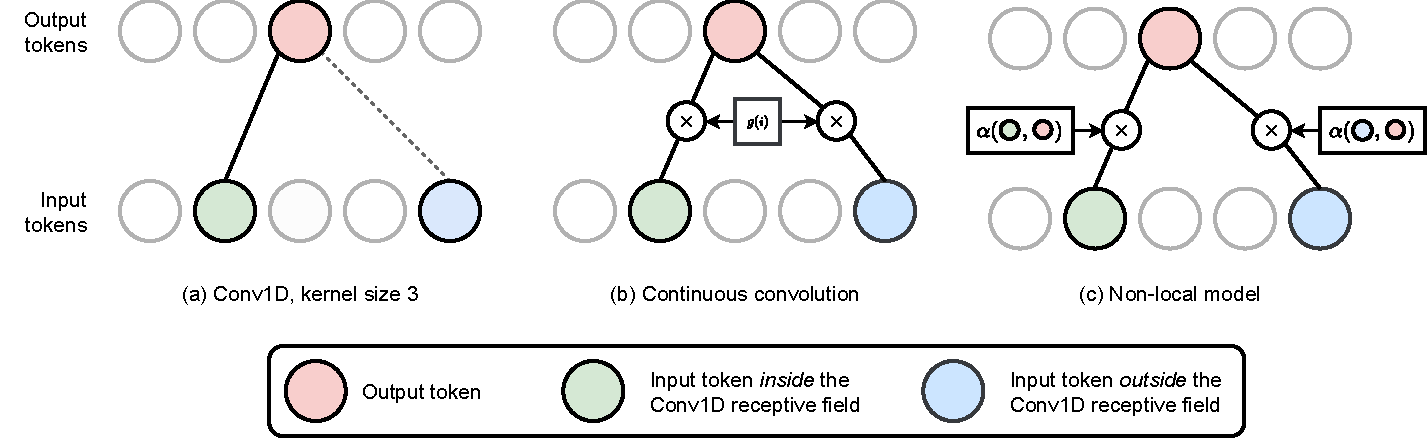
\includegraphics[width=1.0\textwidth]{images/convolution_types}
    \caption{Сравнение различных типов свёрток для 1D-последовательности. Мы показываем, как один выходной токен (в {\color{drawred!30}красном}) взаимодействует с двумя токенами, один внутри рецептивного поля свёртки (в {\color{drawgreen!30}зеленом}), а другой снаружи (в {\color{drawblue!30}синем}). (a) В стандартной свёртке синий токен игнорируется, потому что он находится за пределами рецептивного поля фильтра. (b) Для непрерывной свёртки рассматриваются оба токена, и результирующие весовые матрицы задаются как $g(-1)$ и $g(2)$ соответственно. (c) В нелокальном случае весовые матрицы зависят от попарного сравнения самих токенов.}
    \label{fig:biases}
\end{figure}


Одна из возможностей решить эту проблему заключается в следующем: вместо явного изучения матриц параметров $\mathbf{W}_1, \mathbf{W}_2, \ldots$, мы можем определить их \textit{неявно}, определив отдельный нейронный блок $g(i): \mathbb{R} \rightarrow \mathbb{R}^{e \times e}$, который выводит все весовые матрицы на основе относительного смещения $i$. Следовательно, мы переписываем \eqref{eq:conv_1d} как:

$$
\mathbf{h}_i=\eqnmarkbox[drawred]{node}{\sum_{j=1}^n} g(i-j)\mathbf{x}_j
$$
\annotate[yshift=-1em]{below,right}{node}{Сумма теперь по \textit{всем} токенам}

\vspace{1em}
Это называется \textbf{длинной свёрткой}, поскольку свёртка охватывает всю входную матрицу $\mathbf{X}$. Это также называется \textbf{непрерывной свёрткой} \cite{romero2022towards}, потому что мы можем использовать $g(\cdot)$ для параметризации промежуточных положений или переменных разрешений \cite{romero2022towards}. Количество параметров в этом случае зависит только от параметров $g$, в то время как оно не зависит от $n$, длины последовательности. Определение $g$ нетривиально, потому что оно должно выводить целую весовую матрицу. Мы можем легко восстановить стандартную свёртку:
%
\begin{equation}
    g(i, j) = \begin{cases} \mathbf{W}_{i-j} & \text{ если } \lvert i - j \rvert \le k \\ 0 & \text{ иначе } \end{cases}
\end{equation}
%
Это частично решает проблему дальних зависимостей, но не решает проблему зависимостей, которые зависят от входа, поскольку вес, придаваемый токену, зависит только от относительного смещения по отношению к индексу $i$. Однако эта формулировка предоставляет простой способ решения этой проблемы, позволяя обученной функции $g$ зависеть от \textit{содержимого} токенов, а не от их положений:
%
\begin{equation}
\mathbf{h}_i=\sum_{j=1}^n {\color{drawred}g(\mathbf{x}_i, \mathbf{x}_j)}\mathbf{x}_j
\label{eq:nonlocal_convolution}
\end{equation}
%
В контексте компьютерного зрения эти модели также называются \textbf{нелокальными} сетями \cite{wang2018non}. Мы приводим сравнение стандартных свёрток, непрерывных свёрток и нелокальных свёрток на Рисунке \ref{fig:biases}.

\subsection{Слой внимания} \addclock

Слой MHA является упрощением \eqref{eq:nonlocal_convolution}. Во-первых, работа с функциями, имеющими матричные выходы, сложна, поэтому мы ограничиваем слой работой со скалярными весами. В частности, простой мерой сходства между токенами является их \textbf{скалярное произведение}:
%
$$
g(\mathbf{x}_i, \mathbf{x}_j)=\mathbf{x}_i^\top\mathbf{x}_j
$$
%
Как мы увидим, это приводит к легко распараллеливаемому алгоритму для всей последовательности. Для дальнейшего мы рассмотрим нормализованную версию скалярного произведения:
%
$$
g(\mathbf{x}_i, \mathbf{x}_j)=\frac{1}{\sqrt{e}}\mathbf{x}_i^\top\mathbf{x}_j
$$
%
Это можно мотивировать следующим образом: если мы предположим, что $\mathbf{x}_i \sim \mathcal{N}(0, \sigma^2\mathbf{I})$, дисперсия каждого элемента $\mathbf{x}_i^\top\mathbf{x}_j$ равна $\sigma^4$, следовательно, элементы могут легко расти по величине. Масштабирующий коэффициент гарантирует, что дисперсия скалярного произведения остается ограниченной на уровне $\sigma^2$.

Поскольку мы суммируем по потенциально переменному числу токенов $n$, полезно также включить операцию нормализации, такую как softmax:\footnote{Обозначение $\text{softmax}_j$ в \eqref{eq:pre_self_attention} означает, что мы применяем нормализацию softmax к множеству $\left\{g(\mathbf{x}_i, \mathbf{x}_j)\right\}_{j=1}^n$ независимо для каждого $i$. Это легче увидеть в векторизованном случае, описанном ниже.}
%
\begin{equation}
\mathbf{h}_i=\sum_{j=1}^n {\color{drawgreen}\text{softmax}_j}(g(\mathbf{x}_i, \mathbf{x}_j))\mathbf{x}_j
\label{eq:pre_self_attention}
\end{equation}

В этом контексте мы называем $g(\cdot, \cdot)$ \textbf{функцией оценки внимания}, а выход softmax — \textbf{оценками внимания}. Из-за свойств нормализации softmax мы можем представить, что каждый токен $i$ имеет определенное количество «внимания», которое он может распределить по другим токенам: увеличивая бюджет на одном токене, внимание к другим токенам обязательно уменьшится из-за знаменателя в softmax.

\vspace{-0.5em}
Если мы используем «скалярное произведение внимания», наша функция $g$ не имеет обучаемых параметров. Идея слоя внимания заключается в том, чтобы восстановить их, добавив обучаемые проекции к входу перед вычислением предыдущего уравнения. Для этого мы определяем три обучаемые матрицы ${\color{drawred}\mathbf{W}_k} \sim (k,e)$, ${\color{drawgreen}\mathbf{W}_v} \sim (v,e)$, ${\color{drawblue}\mathbf{W}_q} \sim (k,e)$, где $k$ и $v$ — гиперпараметры. Каждый токен проецируется с помощью этих трех матриц, получая в общей сложности $3n$ токенов:
%
\begin{align}\text{Токены-ключи:} & \quad\;{\color{drawred}\mathbf{k}_i}=\mathbf{W}_k\mathbf{x}_i \label{eq:keys}\\
\text{Токены-значения:} & \quad\; {\color{drawgreen}\mathbf{v}_i}=\mathbf{W}_v\mathbf{x}_i  \label{eq:values}\\
\text{Токены-запросы:} & \quad\; {\color{drawblue}\mathbf{q}_i}=\mathbf{W}_q\mathbf{x}_i\label{eq:queries}\end{align}
%
Эти обработанные токены называются \textbf{ключами}, \textbf{значениями} и \textbf{запросами} (вы можете пока игнорировать выбор терминологии; мы вернемся к этому вопросу в конце раздела). Слой \textbf{самовнимания} (SA) получается путем объединения трех проекций \eqref{eq:keys}-\eqref{eq:values}-\eqref{eq:queries} с \eqref{eq:pre_self_attention}:
%
$$
\mathbf{h}_i=\sum_{j=1}^n \text{softmax}_j(g({\color{drawblue}\mathbf{q}_i}, {\color{drawred}\mathbf{k}_j}))\mathbf{\color{drawgreen}v_j}
$$
%
Следовательно, мы вычисляем обновленное представление токена $i$, сравнивая его запрос со всеми возможными ключами, и используем нормализованные веса для объединения соответствующих токенов-значений. Обратите внимание, что размерность ключей и запросов должна быть одинаковой, в то время как размерность значений может быть разной.

Если мы используем скалярное произведение, мы можем компактно переписать операцию слоя SA для всех токенов. Для этого мы определяем три матрицы со стеком всех возможных ключей, запросов и значений:
%
\begin{align}{\color{drawred}\mathbf{K}}=\mathbf{X}\mathbf{W}_k  \\ {\color{drawgreen}\mathbf{V}}=\mathbf{X}\mathbf{W}_v \\ {\color{drawblue}\mathbf{Q}}=\mathbf{X}\mathbf{W}_q \end{align}
%
Три матрицы имеют форму $(n,k)$, $(n,v)$ и $(n,k)$ соответственно. В качестве примечания, мы также можем реализовать их как одно умножение матриц, выход которого разделен на три части:
%
$$
\begin{bmatrix}\mathbf{K} \\ \mathbf{V} \\  \mathbf{Q} \end{bmatrix} = \mathbf{X}\begin{bmatrix} \mathbf{W}_k  \\ \mathbf{W}_v \\ \mathbf{W}_q \end{bmatrix}
$$
%
Слой SA тогда записывается как:
%
$$
\text{SA}(\mathbf{X})=\text{softmax}\left(\frac{\mathbf{Q}\mathbf{K}^\top}{\sqrt{k}}\right)\mathbf{V}
$$
%
где мы предполагаем, что softmax применяется построчно. Мы также можем сделать проекции явными, как показано ниже.

\begin{definition}[Слой самовнимания] \addbottle
Слой \textbf{самовнимания} (SA) определяется для входа $\mathbf{X} \sim (n,e)$ как:
%
\begin{equation}
\textnormal{SA}(\mathbf{X})=\textnormal{softmax}\left(\frac{\mathbf{X}\mathbf{W}_q\mathbf{W}_k^\top\mathbf{X}^\top}{\sqrt{k}}\right)\mathbf{X}\mathbf{W}_v
\end{equation}
%
Обучаемыми параметрами являются $\mathbf{W}_q \sim (k,e)$, $\mathbf{W}_k \sim (k,e)$ и $\mathbf{W}_v \sim (v,e)$, где $k$ и $v$ — гиперпараметры. Следовательно, имеется $k(2e + v)$ обучаемых параметров, не зависящих от $n$.
%
\end{definition}
%
Мы показываем работу слоя визуально на Рисунке \ref{fig:self_attention}.

\begin{figure}[t]
    \centering
    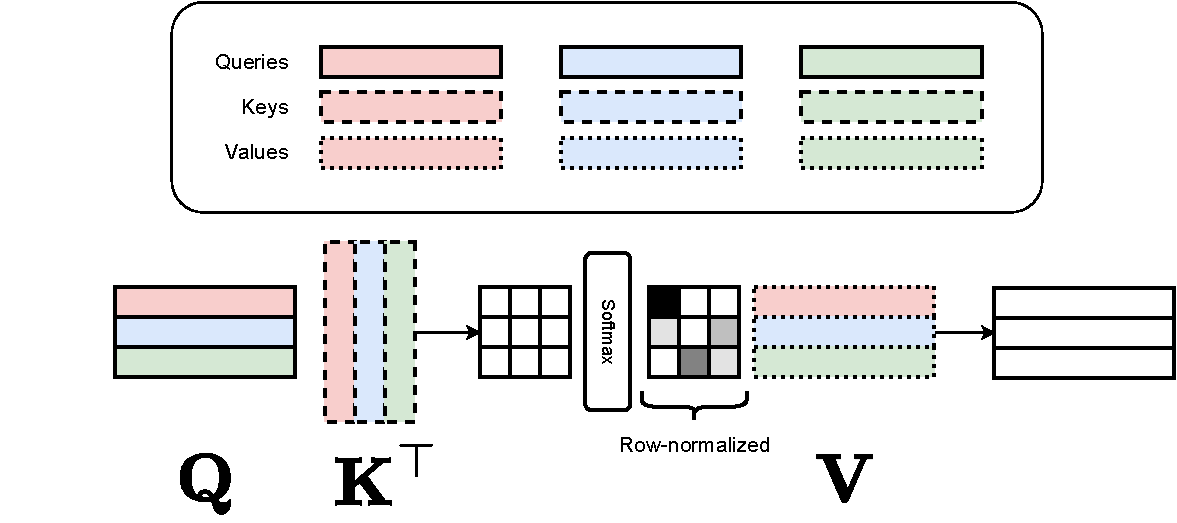
\includegraphics[width=0.9\textwidth]{images/attention-1}
    \caption{Визуализация основных операций слоя SA (за исключением проекций).}
    \label{fig:self_attention}
\end{figure}


\subsection{Многоголовочное внимание}
\label{subsec:multi_head_attention}

Предыдущий слой также называется операцией внимания с \textbf{одной головой}. Он позволяет моделировать попарные зависимости между токенами с высокой гибкостью. Однако в некоторых случаях у нас может быть несколько наборов зависимостей для рассмотрения: снова взяв пример «\textit{кошка, которая принадлежит моей матери, сидит на столе}», зависимости между «\textit{кошкой}» и «\textit{столом}» отличаются от зависимостей между «\textit{кошкой}» и «\textit{матерью}», и мы можем захотеть, чтобы слой мог моделировать их отдельно.\footnote{И все зависит от кошки, конечно.}

Многоголовочный слой достигает этого, запуская несколько операций внимания параллельно, каждая со своим набором обучаемых параметров, перед агрегацией результатов с помощью некоторой операции пулинга. Для этого мы определяем новый гиперпараметр $h$, который мы называем количеством \textbf{голов} слоя. Мы инстанцируем $h$ отдельных проекций для токенов, всего $3hn$ токенов ($3n$ для каждой «головы»):
%
\begin{align}\mathbf{K}_e=\mathbf{X}\mathbf{W}_{k,e} \\ 
\mathbf{V}_e=\mathbf{X}\mathbf{W}_{v,e} \\ 
\mathbf{Q}_e=\mathbf{X} \mathbf{W}_{q,e}
\end{align}
%
$\mathbf{W}_{k,e}$ представляет проекцию ключа для $e$-й головы, и аналогично для других величин. Слой \textbf{многоголовочного внимания} (MHA) выполняет $h$ отдельных операций SA, объединяет результирующие выходные вложения и проецирует их в последний раз в желаемую размерность:

\vspace{1em}
\begin{equation}
\text{MHA}(\mathbf{X})=\begin{bmatrix}\eqnmarkbox[drawred]{node}{\text{softmax}\left(\frac{\mathbf{Q}_1\mathbf{K}_1^\top}{\sqrt{k}}\right)\mathbf{V}_1} \;\mathbin\Vert\; \ldots \; \mathbin\Vert\;\text{softmax}\left(\frac{\mathbf{Q}_h\mathbf{K}_h^\top}{\sqrt{k}}\right)\mathbf{V}_h\end{bmatrix}\eqnmarkbox[drawgreen]{node2}{\mathbf{W}_o}
\label{eq:mha_explicit}
\end{equation}
\annotate[yshift=1em]{above,right}{node}{Отдельный слой SA}
\annotate[yshift=-1em]{below,left}{node2}{Выходная проекция}

\vspace{0.5em}
Каждая операция SA возвращает матрицу формы $(n,v)$. Эти $h$ матриц объединяются по второму измерению, чтобы получить матрицу $(n,hv)$, которая затем проецируется с помощью матрицы $\mathbf{W}_o \sim (o,hv)$, где $o$ — дополнительный гиперпараметр, обеспечивающий гибкость в выборе выходной размерности.

\subsection*{Объяснение терминологии} 

Чтобы понять, почему три токена называются запросами, ключами и значениями, \addteacup мы рассмотрим аналогию слоя SA со стандартным словарем Python, который показан в Листинге \ref{code:dictionary}. 

\begin{mypy}{Словарь в Python: значение возвращается только в том случае, если найдено точное совпадение ключа и запроса. В противном случае мы получаем ошибку.}{code:dictionary}
d = dict()
d["Симоне"] = 2
d["Симоне"]       # Возвращает 2
d["Смоне "]       # Возвращает ошибку
\end{mypy}

Формально, словарь — это набор пар вида (ключ, значение), где ключ действует как уникальный идентификатор для извлечения соответствующего значения. Например, в третьей и четвертой строках Листинга \ref{code:dictionary} мы запрашиваем словарь с двумя разными строками («\textit{Симоне}» и «\textit{Смоне }»): словарь сравнивает строку запроса со всеми ключами, которые хранятся внутри, возвращая соответствующее значение, если найдено точное совпадение, и ошибку в противном случае.

Для меры сходства пар ключей мы можем рассмотреть вариант стандартного словаря, который всегда возвращает значение, соответствующее ближайшему ключу, найденному в словаре. Если ключи, запросы и значения являются векторами, этот вариант словаря эквивалентен нашему слою SA, если мы заменим операцию softmax на argmax по токенам, как показано на Рисунке \ref{fig:hard_attention}.

Этот «жесткий» вариант внимания трудно реализовать, потому что градиенты операции argmax почти везде равны нулю (мы рассмотрим дискретную выборку и аппроксимацию операции argmax с помощью дискретной релаксации в следующем томе). Следовательно, мы можем интерпретировать слой SA как мягкую аппроксимацию, в которой каждый токен обновляется взвешенной комбинацией всех значений на основе соответствующих сходств ключ/запрос.

\begin{figure}[t]
    \centering
    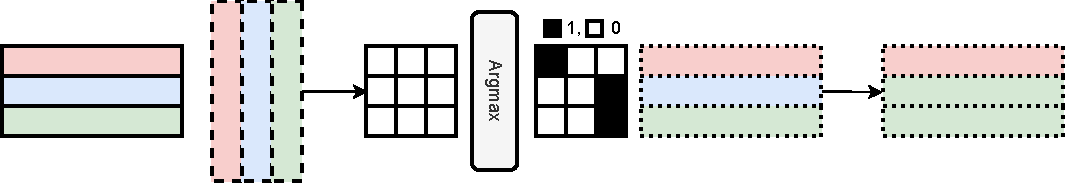
\includegraphics[width=1.0\textwidth]{images/attention-2}
    \caption{SA с «жестким» вниманием эквивалентен векторнозначному словарю.}
    \label{fig:hard_attention}
\end{figure}

\begin{supportbox}{Головы и схемы}

Вскоре мы увидим, что слой MHA всегда комбинируется с остаточным соединением (Раздел \ref{sec:residual_connections}). В этом случае мы можем записать его выход для $i$-го токена как:

\vspace{2em}
\begin{equation}
\mathbf{x}_i \leftarrow \mathbf{x}_i + \eqnmarkbox[drawred]{node}{\sum_e} \eqnmarkbox[drawgreen]{node2}{\sum_j} \alpha_e(\mathbf{x}_i, \mathbf{x}_j)\mathbf{W}_e^\top \mathbf{x}_j
\end{equation}
\annotate[yshift=1em]{above,right}{node}{Сумма по головам}
\annotate[yshift=-1em]{below,right}{node2}{Сумма по токенам}

\vspace{2em}
где $\alpha_e(\mathbf{x}_i, \mathbf{x}_j)$ — это оценка внимания между токенами $i$ и $j$ в голове $e$, а $\mathbf{W}_e$ объединяет проекцию значения $e$-й головы с $e$-м блоком выходной проекции в \eqref{eq:mha_explicit}. Вложения токенов иногда называют \textbf{остаточным потоком} модели.\footnote{Это было популяризировано в контексте \textbf{механистической интерпретируемости}, которая пытается реконструировать поведение слоев, чтобы найти интерпретируемые компоненты, называемые \textit{схемами}: \url{https://transformer-circuits.pub}. Линейность потока является фундаментальной для анализа.} Следовательно, головы можно понимать как «чтение» из остаточного потока (через проекцию $\mathbf{W}_e$ и выбор через оценки внимания) и линейное «записывание» обратно в потоки.
\end{supportbox}

\section{Позиционные вложения}
\label{sec:positional_embeddings}

Имея слой MHA, мы рассмотрим проектирование полной модели трансформера, которая требует еще одного компонента, позиционных вложений.

\subsection{Перестановочная эквивариантность слоя MHA}

Интересно рассмотреть, что происходит с выходом слоя MHA, когда порядок токенов переупорядочивается (\textit{переставляется}). Чтобы формализовать это, мы вводим понятие \textbf{матриц перестановок}.

\begin{definition}[Матрица перестановки]
\textbf{Матрица перестановки} размера $n$ — это квадратная бинарная матрица $\mathbf{P} \sim \text{Binary}(n,n)$, такая, что в каждой строке или столбце присутствует только одна $1$:

$$
\mathbf{1}^\top\mathbf{P}=\mathbf{1},\;\; \mathbf{P}\mathbf{1}=\mathbf{1}
$$

Если мы уберем требование, чтобы матрица имела двоичные элементы, и ограничим элементы только неотрицательными, мы получим множество \textbf{дважды стохастических} матриц (матриц, у которых строки и столбцы суммируются в единицу).

\end{definition}

Эффект применения матрицы перестановки заключается в переупорядочивании соответствующих строк/столбцов матрицы. Например, рассмотрим следующую перестановку:

$$
\mathbf{P}=\begin{bmatrix} 1 & 0 & 0 \\ 0 & 0 & 1 \\ 0 & 1 & 0 \end{bmatrix}
$$

Глядя на строки, мы видим, что второй и третий элементы меняются местами при ее применении:

$$
\mathbf{P}\begin{bmatrix} {\color{drawred}\mathbf{x}_1} \\ {\color{drawgreen}\mathbf{x}_2} \\ {\color{drawblue}\mathbf{x}_3} \end{bmatrix} = \begin{bmatrix} {\color{drawred}\mathbf{x}_1} \\ {\color{drawblue}\mathbf{x}_3}  \\ {\color{drawgreen}\mathbf{x}_2}\end{bmatrix}
$$

Интересно, что единственным эффектом применения матрицы перестановки к входам слоя MHA является переупорядочивание выходов слоя эквивалентным образом:

$$
\text{MHA}(\mathbf{P}\mathbf{X})=\mathbf{P}\,\cdot\,\text{MHA}(\mathbf{X})
$$

\begin{figure}[t]
    \centering
    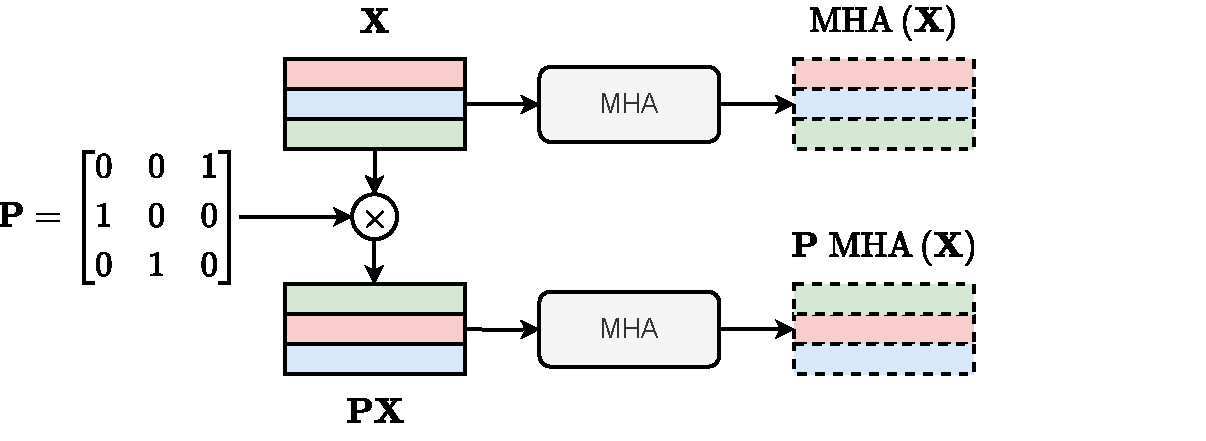
\includegraphics[width=0.95\textwidth]{images/permutation_equivariance}
    \caption{Выход слоя MHA после перестановки порядка токенов тривиально является перестановкой исходных выходов.}
    \label{fig:permutation_equivariance_mha}
\end{figure}

Это немедленно доказывается. Мы сосредоточимся на варианте с одной головой, поскольку вариант с несколькими головами аналогичен. Во-первых, softmax перенормирует элементы по столбцам матрицы, поэтому он тривиально перестановочно эквивариантен как по строкам, так и по столбцам:

$$
\text{softmax}(\mathbf{P}\mathbf{X}\mathbf{P}^\top)=\mathbf{P}\left[\text{softmax}(\mathbf{X})\right]\mathbf{P}^\top
$$

Из этого мы можем немедленно вывести позиционную эквивариантность SA:

\begin{gather}
\text{SA}(\mathbf{P}\mathbf{X}) = \text{softmax}\left(\mathbf{P}\frac{\mathbf{X}\mathbf{W}_q\mathbf{W}_k^\top\mathbf{X}^\top}{\sqrt{k}}\mathbf{P}^\top\right)\mathbf{P}\mathbf{X}\mathbf{W}_v \\
= \mathbf{P}\text{softmax}\left(\frac{\mathbf{X}\mathbf{W}_q\mathbf{W}_k^\top\mathbf{X}^\top}{\sqrt{k}}\right)\mathbf{X}\mathbf{W}_v = \mathbf{P}\cdot\text{SA}(\mathbf{X})
\end{gather}

где мы используем тот факт, что $\mathbf{P}^\top \mathbf{P} = \mathbf{I}$ для любой матрицы перестановки. Это также можно увидеть, рассуждая о слое SA для каждого токена: выход задается суммой элементов, каждый из которых взвешен попарным сравнением. Следовательно, для данного токена операция является \textbf{перестановочно инвариантной}. Вместо этого, для всей входной матрицы операция является \textbf{перестановочно эквивариантной}.

Трансляционная эквивариантность была желательным свойством для свёрточного слоя, но перестановочная эквивариантность \textit{нежелательна} (по крайней мере, здесь), потому что она отбрасывает ценный порядок входной последовательности. В качестве примера, единственным эффектом обработки текста, токены которого были перевернуты, будет переворот выхода слоя, несмотря на то, что результирующий перевернутый вход, вероятно, недействителен. Формально, слои SA и MHA являются функциями множеств, а не функциями последовательностей.

Вместо того, чтобы изменять слой или добавлять слои, которые не являются перестановочно эквивариантными, трансформер работает, вводя новую концепцию \textbf{позиционных вложений}, которые являются вспомогательными токенами, зависящими только от положения токена в последовательности (\textbf{абсолютные позиционные вложения}) или смещения двух токенов (\textbf{относительные позиционные вложения}). Мы опишем их по очереди.

\subsection{Абсолютные позиционные вложения}

Каждый токен во входной матрице $\mathbf{X} \sim (n,e)$ представляет \textit{содержимое} конкретного фрагмента текста (например, подслова). Предположим, мы фиксируем максимальную длину любой последовательности в $m$ токенов. Чтобы преодолеть перестановочную эквивариантность, мы вводим дополнительный набор \textbf{позиционных вложений} $\mathbf{S} \sim (m,e)$, где вектор $\mathbf{S}_i$ однозначно кодирует понятие «находиться в позиции $i$». Следовательно, сумма входной матрицы с первыми строками $\mathbf{S}$:
%
$$
\mathbf{X}^\prime =  \mathbf{X} + \mathbf{S}_{1:n}
$$
%
такова, что $\idx{\mathbf{X}^\prime}{i}$ представляет «токен $\mathbf{X}_i$ в позиции $i$».
%
Поскольку нет смысла переставлять позиционные вложения (поскольку они зависят только от положения), результирующий слой больше не является перестановочно эквивариантным:
%
$$
\text{MHA}(\mathbf{P}\mathbf{X} + \mathbf{S}) \neq \mathbf{P}\,\cdot\,\text{MHA}(\mathbf{X}+\mathbf{S})
$$
%
См. Рисунок \ref{fig:positional_embeddings} для визуализации этой идеи. 

\begin{SCfigure}[1.5]
    \centering
    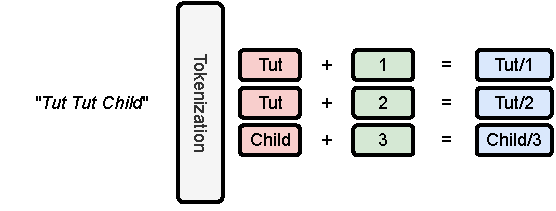
\includegraphics[width=0.6\textwidth]{images/positional_embeddings}
    \caption{Позиционные вложения ({\color{drawgreen!30}зеленый}) добавляются к вложениям токенов ({\color{drawred!30}красный}). Один и тот же токен в разных позициях имеет разные выходы ({\color{drawblue!30}синий}).}
    \label{fig:positional_embeddings}
\end{SCfigure}

Как нам построить позиционные вложения? Самая простая стратегия — рассматривать $\mathbf{S}$ как часть параметров модели и обучать его вместе с остальными обучаемыми параметрами, аналогично вложениям токенов. Эта стратегия хорошо работает, когда количество токенов относительно стабильно; мы увидим пример в следующей главе в контексте компьютерного зрения.

В качестве альтернативы мы можем определить некоторую детерминированную функцию из множества позиций токенов в заданный вектор, который однозначно идентифицирует позицию. Некоторые стратегии явно являются плохим выбором, например:
%
\begin{enumerate}
\item Мы можем связать с каждой позицией скаляр $p=i/m$, который линейно возрастает с позицией. Однако добавление одного скаляра к вложениям токенов оказывает незначительное влияние.
\item Мы можем one-hot закодировать позицию в двоичный вектор размера $m$, но результирующий вектор будет чрезвычайно разреженным и высокоразмерным.
\end{enumerate}
%
Возможность, представленная в оригинальной статье о трансформере \cite{vaswani2017attention}, — это \textbf{синусоидальные вложения}. Чтобы понять их, рассмотрим синусоидальную функцию:
%
$$
y=\sin(x)
$$
%
Синус присваивает уникальное значение любому входу $x$ в диапазоне $[0, 2\pi]$. Мы также можем изменять частоту синуса:
%
$$
y=\sin(\omega x)
$$
%
Он колеблется более или менее быстро в зависимости от частоты $\omega$ и присваивает уникальное значение любому входу в диапазоне $[0, \frac{2\pi}{\omega}]$. Существует аналогия с (аналоговыми) часами: секундная стрелка совершает полный оборот с частотой $\frac{1}{60}$ Гц (один раз в минуту). Следовательно, каждый «момент времени» в течение минуты можно различить, глядя на стрелку, но два момента времени в общем можно идентифицировать только с точностью до 60 секунд. Мы преодолеваем это в часах, добавляя отдельную стрелку (минутную), которая вращается с гораздо меньшей частотой $\frac{1}{3600}$ Гц. Следовательно, глядя на пару координат (секунда, минута) («вложение» времени), мы можем различить любую точку в течение часа. Добавляя еще одну стрелку с еще меньшей частотой (часовую), мы можем различить любую точку в течение дня. Это можно обобщить: мы могли бы спроектировать часы с более низкими или более высокими частотами для различения месяцев, лет или миллисекунд.

Аналогичную стратегию можно применить и здесь: мы можем различать каждую позицию $i$, кодируя ее через набор из $e$ синусов (где $e$ — гиперпараметр) с возрастающими частотами:
%
$$
\mathbf{S}_i=\left[ \sin(\omega_1i), \sin(\omega_2i),\ldots,\sin(\omega_ei) \right]
$$
%
На практике исходное предложение из \cite{vaswani2017attention} использует только $e/2$ возможных частот, но добавляет как синусы, так и косинусы:
%
$$
\mathbf{S}_i=\left[ \sin(\omega_1i), \cos(\omega_1i),\sin(\omega_2i), \cos(\omega_2i),\ldots,\sin(\omega_{e/2}i), \cos(\omega_{e/2}i) \right]
$$
%
Это можно оправдать, заметив, что в этом вложении две позиции связаны простым линейным преобразованием, вращением, которое зависит только от относительного смещения двух позиций.\footnote{См. \url{https://kazemnejad.com/blog/transformer_architecture_positional_encoding/} для подробного вычисления.} Любой выбор частоты действителен при условии, что они достаточно велики и возрастают со сверхлинейной скоростью. Выбор из \cite{vaswani2017attention} был геометрической прогрессией:
%
$$
\omega_i=\frac{1}{10000^{i/e}}
$$
%
которая изменяется от $\omega_0=1$ до $\omega_e=\frac{1}{10000}$. См. Рисунок \ref{fig:positional_embeddings_plot} для визуализации.

\begin{SCfigure}
    \centering
    \hspace{1em}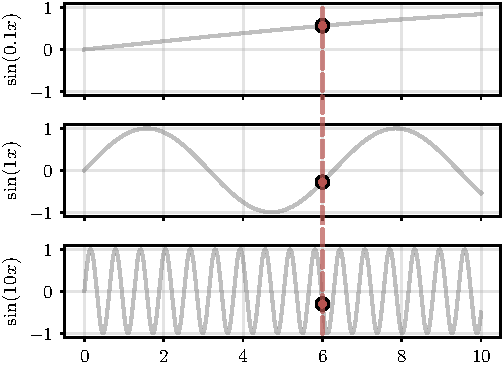
\includegraphics[width=0.6\textwidth]{images/positional_embeddings_plot}
    \caption{Мы показываем три функции $\sin$ с $\omega=0.1$, $\omega=1$ и $\omega=10$. Вложение для позиции $x=6$ задается соответствующими значениями (красные круги).}
    \label{fig:positional_embeddings_plot}
\end{SCfigure}

\subsection{Относительные позиционные вложения}

Обучаемые позиционные вложения и синусоидальные позиционные вложения являются примерами \textbf{абсолютных} вложений, поскольку они кодируют конкретную позицию в последовательности. Альтернативой, которая стала распространенной для очень длинных последовательностей, являются \textbf{относительные позиционные вложения}. В этом случае вместо добавления позиционного кодирования к токену мы изменяем функцию внимания, чтобы сделать ее зависимой от смещения между любыми двумя токенами:
%
$$
g(\mathbf{x}_i, \mathbf{x}_j)\rightarrow g(\mathbf{x}_i, \mathbf{x}_j, i-j)
$$
%
Это комбинация двух идей, которые мы представили в начале этой главы (Рисунок \ref{fig:biases}). Обратите внимание, что в то время как абсолютные вложения добавляются только один раз (на входе), относительные вложения должны добавляться каждый раз, когда используется слой MHA. В качестве примера мы можем добавить обучаемую матрицу смещения $\mathbf{B} \sim (m,m)$ и переписать скалярное произведение со смещением, зависящим от смещения:
%
$$
g(\mathbf{x}_i,\mathbf{x}_j)=\mathbf{x}_i^\top\mathbf{x}_j+B_{ij}
$$
%
Более простой вариант, \textbf{внимание с линейными смещениями} (ALiBi) \cite{press2021train}, рассматривает один обучаемый скаляр в каждой голове, который умножается на матрицу смещений. Возможны и более продвинутые стратегии, такие как \textbf{ротационные позиционные вложения} (RoPE) \cite{su2024roformer}.

\section{Построение модели трансформера}
\subsection{Блок и модель трансформера}
\label{subsec:transformer_block}

В принципе, модель можно было бы построить из стека нескольких слоев MHA (с softmax, обеспечивающим нелинейность, необходимую для предотвращения схлопывания нескольких линейных проекций). Однако эмпирически было обнаружено, что MHA лучше всего работает, когда чередуется с отдельным полносвязным блоком, который работает с каждым токеном независимо. Эти две операции можно понимать как смешивание токенов (MHA) и смешивание каналов (MLP), аналогично модели глубинно-разделимой свёртки.

В частности, для блока MLP обычно выбирают архитектуру бутылочного горлышка, состоящую из двух полносвязных слоев вида:
%
$$
\text{MLP}(\mathbf{x})=\mathbf{W}_2\phi\left(\mathbf{W}_1\mathbf{x}\right)
$$
%
где $\mathbf{x} \sim (e)$ — это токен, $\mathbf{W}_1 \sim (p, e)$, где $p$ выбирается как целое кратное $e$ (например, $p=3e$ или $p=4e$), а $\mathbf{W}_2 \sim (e,p)$ перепроецирует обратно в исходную размерность вложения. Смещения обычно удаляются, поскольку увеличенная скрытая размерность обеспечивает достаточные степени свободы.

Чтобы обеспечить эффективное обучение глубоких моделей, нам также нужны несколько дополнительных стратегий регуляризации. В частности, обычно включают два шага послойной нормализации и два остаточных соединения, соответственно для блоков MHA и MLP. В зависимости от того, где применяется послойная нормализация, мы получаем два варианта базового блока трансформера, иногда обозначаемые как \textbf{предварительно нормализованный} и \textbf{пост-нормализованный}. Они показаны на Рисунке \ref{fig:pre_post_normalization}.

\begin{SCfigure}
    \centering
    \hspace{2em}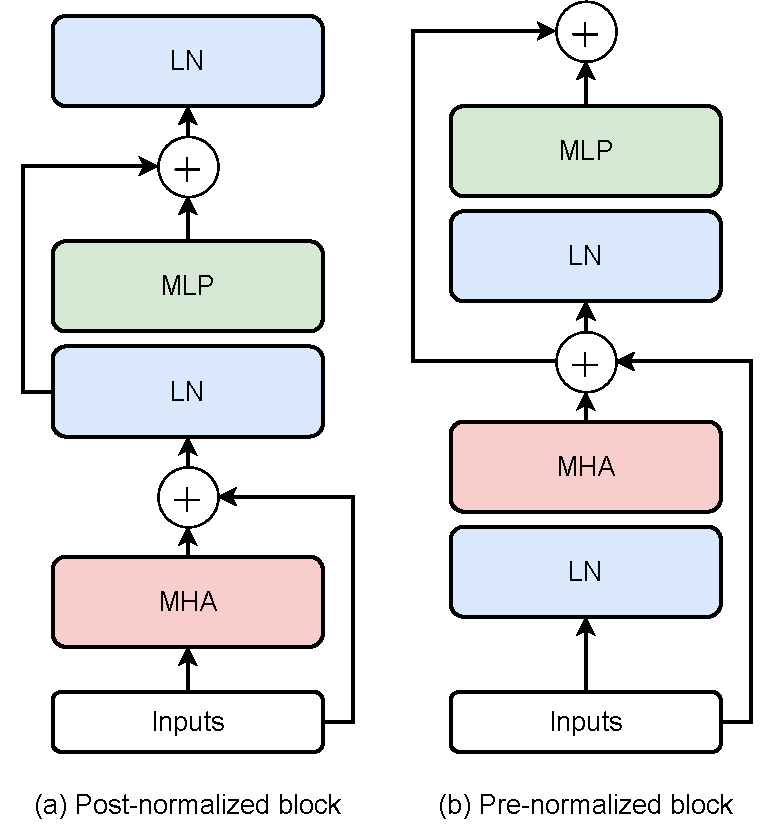
\includegraphics[width=0.4\textwidth]{images/transformer_block}
    \caption{Схематический вид предварительно нормализованных и пост-нормализованных блоков трансформера. В пост-нормализованном варианте блок LN применяется после операции MHA или MLP, в то время как в предварительно нормализованном — перед каждым слоем.}
    \label{fig:pre_post_normalization}
\end{SCfigure}

Хотя пост-нормализованная версия соответствует оригинальному блоку трансформера, предварительно нормализованный вариант, как правило, оказывается более стабильным и быстрым в обучении \cite{xiong2020layer}. Дизайн блока на Рисунке \ref{fig:pre_post_normalization} является, по сути, эмпирическим выбором, и в литературе было предложено и протестировано множество вариантов. Мы рассмотрим некоторые из них позже в Разделе \ref{subsec:mha_variants}.

Теперь мы можем завершить описание базовой модели трансформера:
%
\begin{enumerate}
\item Токенизировать и вложить исходную входную последовательность в матрицу $\mathbf{X} \sim (n,e)$.\\
\item Если используются абсолютные позиционные вложения, добавить их к входной матрице.
\item Применить 1 или более блоков вида, описанного выше.
\item Включить заключительную голову в зависимости от задачи.
\end{enumerate}
%
Выход шага (3) — это набор обработанных токенов $\mathbf{H} \sim (n,e)$, где ни $n$, ни $e$ не изменяются моделью трансформера (первое, потому что у нас нет локальных операций пулинга на множествах, второе — из-за остаточных соединений в блоке). Рассматривая, например, задачу классификации, мы можем применить стандартную классификационную голову, выполнив пулинг по токенам и продолжив с полносвязным блоком:
%
$$
y=\text{softmax}\left(\text{MLP}\left(\frac{1}{n}\sum_i\mathbf{H}_i\right)\right)
$$
%
Эта часть идентична соответствующему дизайну СНС. Однако у трансформера есть ряд интересных свойств, в основном вытекающих из того факта, что он манипулирует своим входом как множеством, не изменяя его размерность на протяжении всей архитектуры. Мы рассмотрим один простой пример далее.

\subsection{Классовые токены и токены-регистры}
\label{subsec:class_register_tokens}

Хотя до сих пор мы предполагали, что каждый токен соответствует одной части нашей входной последовательности, ничто не мешает нам добавлять \textit{дополнительные} токены к входу трансформера. Это строго зависит от его конкретной архитектуры: СНС, например, требует, чтобы ее вход был точно упорядочен, и неясно, как мы могли бы добавить дополнительные токены к изображению или последовательности. Это очень мощная идея, и мы рассмотрим здесь только две конкретные реализации.

Во-первых, мы рассмотрим использование \textbf{классового токена} \cite{dosovitskiy2020image}, дополнительного токена, который добавляется явно для классификации, чтобы заменить операцию глобального пулинга выше. Предположим, мы инициализируем один обучаемый токен $\mathbf{c} \sim (e)$, который добавляется к входной матрице:
%
$$
\mathbf{X} \leftarrow\begin{bmatrix}\mathbf{X} \\ \mathbf{c}^\top \end{bmatrix}
$$
%
Новая матрица имеет форму $(n+1, e)$. Классовый токен идентичен для всех последовательностей в мини-пакете. После шага (3) выше, трансформер выводит матрицу $\mathbf{H} \sim (n+1,e)$ обновленных представлений для всех токенов, включая классовый. Идея заключается в том, что вместо пулинга по токенам модель должна быть в состоянии «сжать» всю информацию, связанную с задачей классификации, внутри классового токена, и мы можем переписать классификационную голову, просто отбросив все остальные токены:\footnote{На языке схем и голов из Раздела \ref{subsec:multi_head_attention} мы могли бы эквивалентно сказать, что модель должна научиться перемещать всю информацию, связанную с классификацией, в остаточный поток классового токена.}
%
$$
y=\text{softmax}\left(\text{MLP}\left(\mathbf{H}_{n+1}\right)\right)
$$
%
Дополнительные обучаемые токены могут быть полезны, даже если они не используются явно. Например, \cite{darcet2023vision} показали, что добавление нескольких дополнительных токенов (называемых в этом случае \textbf{регистрами}) может улучшить качество карт внимания, предоставляя модели возможность использовать регистры для «хранения» вспомогательной информации, которая не зависит явно от данной позиции.

\section*{От теории к практике}

\begin{wrapfigure}{r}{3.0cm}
\vspace{-6em}
\includegraphics[width=3.0cm]{images/shutterstock_2075221579.jpg}
\vspace{-4em}
\end{wrapfigure}

В следующей главе мы представим много важных понятий, связанных с трансформерами. Поэтому для этой главы я предлагаю немного нетрадиционное упражнение, которое сочетает в себе свёрточную основу с головой, подобной трансформеру, как показано на Рисунке \ref{fig:multiview_model}.

\begin{figure}[t]
    \centering
    \hspace{1em}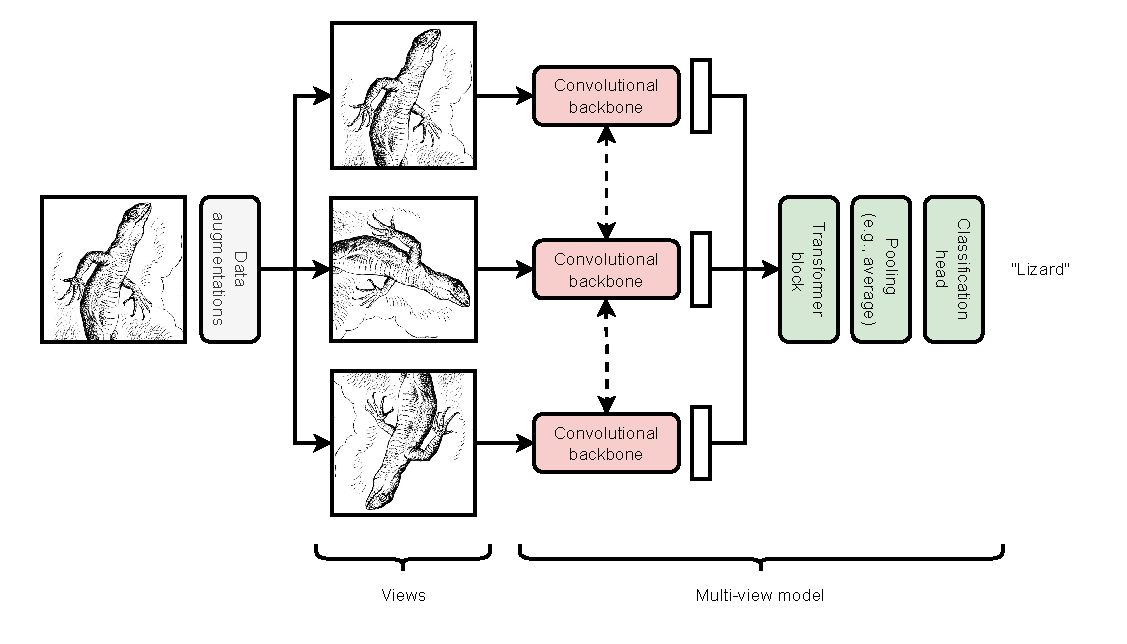
\includegraphics[width=1\textwidth]{images/Multiviewmodel}
    \caption{Многовидовая модель для реализации в этой главе. Изображение аугментируется с помощью набора случайных стратегий аугментации данных для получения набора \textbf{видов} входа ({\color{gray!30}серый}). Каждый \textit{вид} обрабатывается одной и той же свёрточной основой для получения вложения фиксированного размера ({\color{drawred!30}красный}). Набор вложений обрабатывается блоком трансформера перед окончательной классификацией ({\color{drawgreen!30}зеленый}). Иллюстрация Джона Тенниела.}
    \label{fig:multiview_model}
\end{figure}

Свёрточные модели, которые вы разработали в Главах \ref{chap:cnns} и \ref{chap:deep_cnns}, применялись к \textit{одному} изображению. Однако иногда у нас есть \textit{набор} изображений одного и того же объекта для распознавания — например, в системе мониторинга у нас может быть несколько скриншотов подозрительного человека. В литературе это называется \textbf{многовидовой} системой, и каждое изображение называется \textbf{видом} объекта. Многовидовая модель должна давать одно предсказание для всего набора видов, будучи инвариантной к порядку видов на входе. В этом упражнении мы реализуем простую многовидовую модель — см. Рисунок \ref{fig:multiview_model}.

\begin{enumerate}
\item Используя любой набор данных для классификации изображений, вы можете смоделировать многовидовую модель, применив фиксированное количество преобразований данных к входу (серый блок на Рисунке \ref{fig:multiview_model}). Игнорируя измерение пакета, для каждого входного изображения формы $x \sim (h,w,c)$ (высота, ширина, каналы) вы получаете \textit{многовидовой} вход формы $x^\prime \sim (v,h,w,c)$, где $v$ — количество видов. С этим тензором связана одна метка $y$ — метка исходного изображения. Количество видов также может отличаться от мини-пакета к мини-пакету, поскольку ни одна часть модели не ограничена заранее заданным количеством видов.
\item Многовидовая модель состоит из трех компонентов. Обозначим через $g(x)$ модель, которая обрабатывает один вид в вложение фиксированного размера — например, это может быть любая свёрточная основа, которую вы обучили для предыдущих упражнений. Первая часть полной модели (красная часть на Рисунке \ref{fig:multiview_model}) применяет $g$ параллельно ко всем видам, $\mathbf{h}_i = g(x_i) \sim (e)$, где $e$ — гиперпараметр (размер выхода основы).
\item После объединения вложений видов мы получаем матрицу $\mathbf{H} \sim (v, e)$. Чтобы полная модель была перестановочно инвариантной, любой компонент, применяемый к $\mathbf{H}$, должен быть перестановочно эквивариантным.\footnote{Операция среднего по видам является простейшим примером перестановочно инвариантного слоя. Следовательно, удаление блока MHA с Рисунка \ref{fig:multiview_model} также является допустимой базовой линией. В качестве альтернативы, глубокие множества \cite{zaheer2017deep} характеризуют полный спектр линейных, перестановочно инвариантных слоев.} Для целей этого упражнения реализуйте и примените один блок трансформера согласно Разделу \ref{subsec:transformer_block}. Вы можете реализовать MHA, используя базовый PyTorch, или вы можете попробовать более продвинутую реализацию с использованием \texttt{einops}.\footnote{См. \url{https://einops.rocks/pytorch-examples.html}.} Вы также можете сравнить с предварительно реализованной версией в \mintinline{python}{torch.nn}.
\item Блок трансформера не изменяет форму входа. Чтобы завершить модель, выполните усреднение по видам (которые представляют токены в этом сценарии) и примените заключительную классификационную голову. Вы также можете поэкспериментировать с добавлением классового токена (Раздел \ref{subsec:class_register_tokens}). Легко показать, что модель, построенная таким образом, является перестановочно инвариантной по отношению к видам.
\end{enumerate}
